We demonstrate the phase-transition phenomena with numerical experiments.

\subsection{The strong classification boundary in finite dimensions}

The sparsity and signal size of the sparse mean vector are parametrized as in \eqref{eq:signal-sparsity} and \eqref{eq:signal-size}, and signal sizes are assumed  equal.
We estimate the support set $S$ with using Bonferroni's procedure, where the nominal FWER level for Bonferroni's procedures are set at $1/(5{\log{p}})$, in line with the assumptions in Theorem \ref{thm:chi-squred-strong-boundary}.
Experiments were repeated 1000 times at each of the 400 sparsity-and-signal-size combinations, and for dimensions 100, 1000, and 10000.

The empirical probabilities of exact support recovery under Bonferroni's procedure are shown in Figure \ref{fig:phase-simulated-chi-squared}.
The numerical results suggest that the predicted boundaries are reasonably accurate in high-dimensions ($p=10000$, right panels of Figure \ref{fig:phase-simulated-chi-squared}), and relevant even at moderate dimensions ($p=100$, left panels of Figure \ref{fig:phase-simulated-chi-squared}).

\begin{figure}
      \centering
      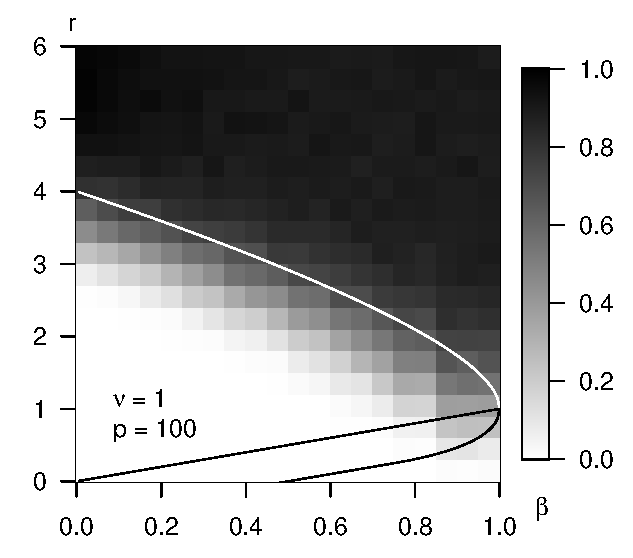
\includegraphics[width=0.32\textwidth]{./sim_strong_boundary/simulated_phase_diagram_chi-squared_nu1_p100.eps}
      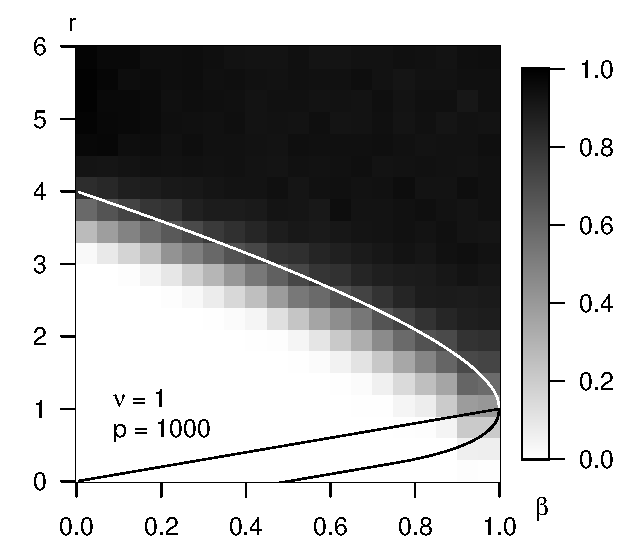
\includegraphics[width=0.32\textwidth]{./sim_strong_boundary/simulated_phase_diagram_chi-squared_nu1_p1000.eps}
      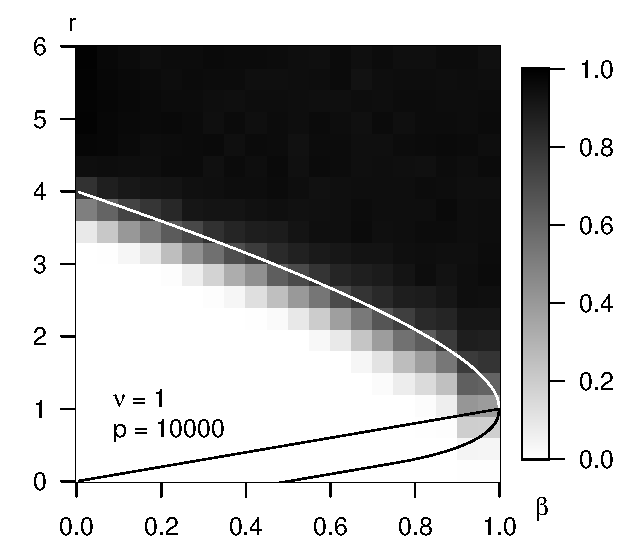
\includegraphics[width=0.32\textwidth]{./sim_strong_boundary/simulated_phase_diagram_chi-squared_nu1_p10000.eps}
      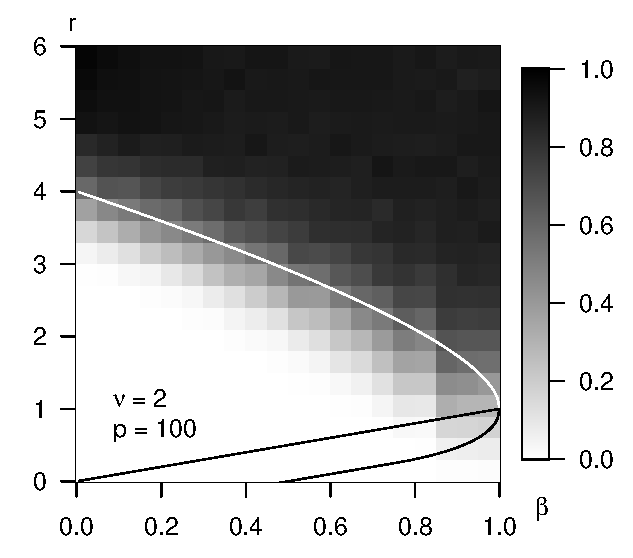
\includegraphics[width=0.32\textwidth]{./sim_strong_boundary/simulated_phase_diagram_chi-squared_nu2_p100.eps}
      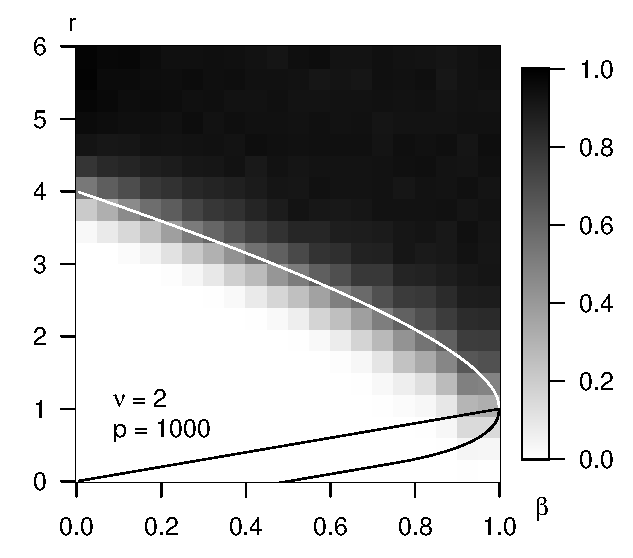
\includegraphics[width=0.32\textwidth]{./sim_strong_boundary/simulated_phase_diagram_chi-squared_nu2_p1000.eps}
      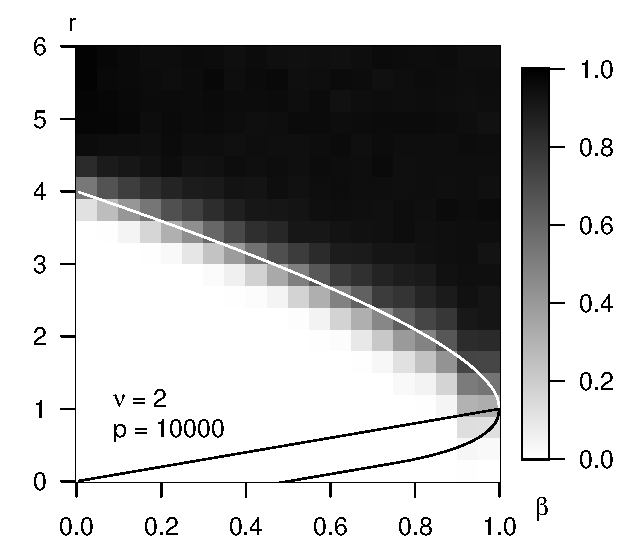
\includegraphics[width=0.32\textwidth]{./sim_strong_boundary/simulated_phase_diagram_chi-squared_nu2_p10000.eps}
      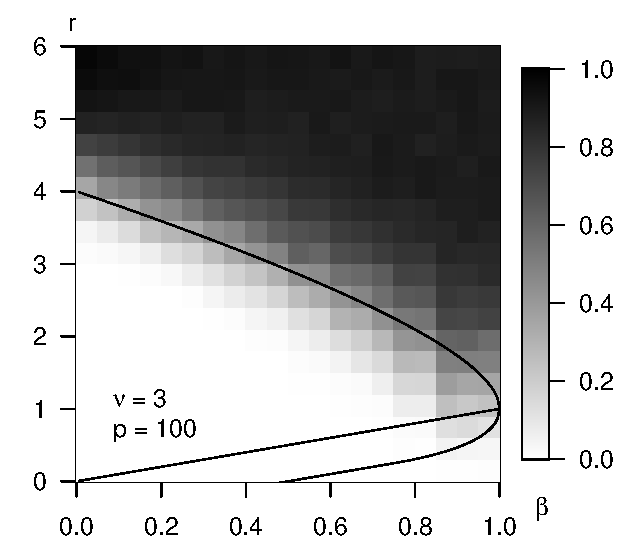
\includegraphics[width=0.32\textwidth]{./sim_strong_boundary/simulated_phase_diagram_chi-squared_nu3_p100.eps}
      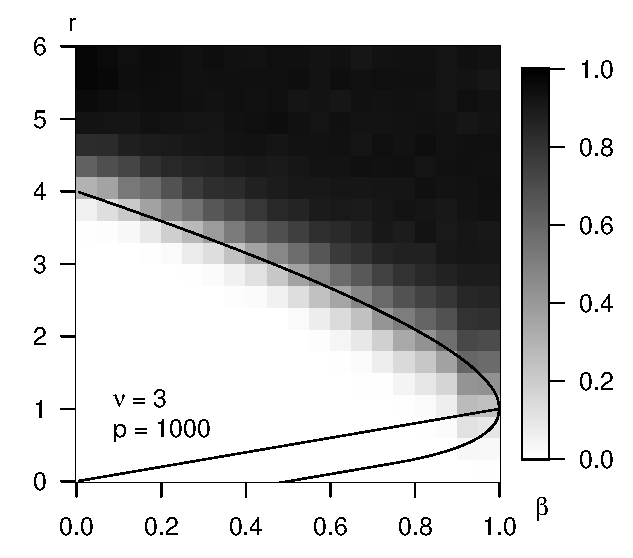
\includegraphics[width=0.32\textwidth]{./sim_strong_boundary/simulated_phase_diagram_chi-squared_nu3_p1000.eps}
      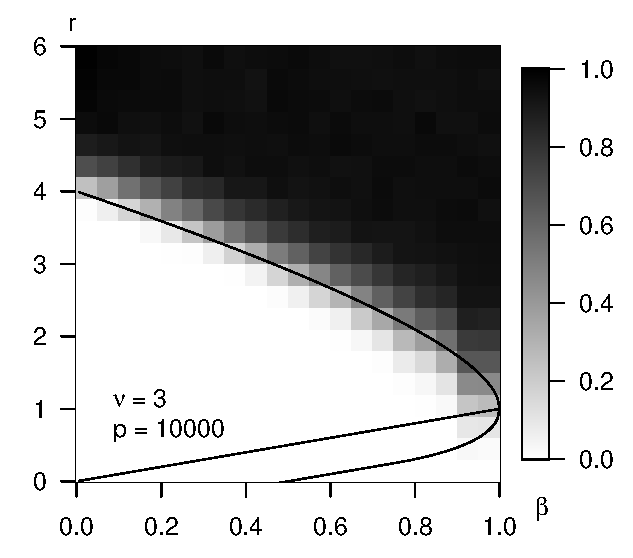
\includegraphics[width=0.32\textwidth]{./sim_strong_boundary/simulated_phase_diagram_chi-squared_nu3_p10000.eps}
      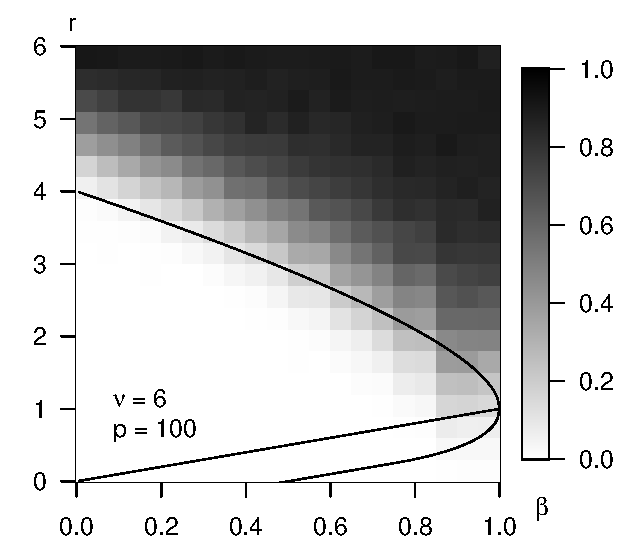
\includegraphics[width=0.32\textwidth]{./sim_strong_boundary/simulated_phase_diagram_chi-squared_nu6_p100.eps}
      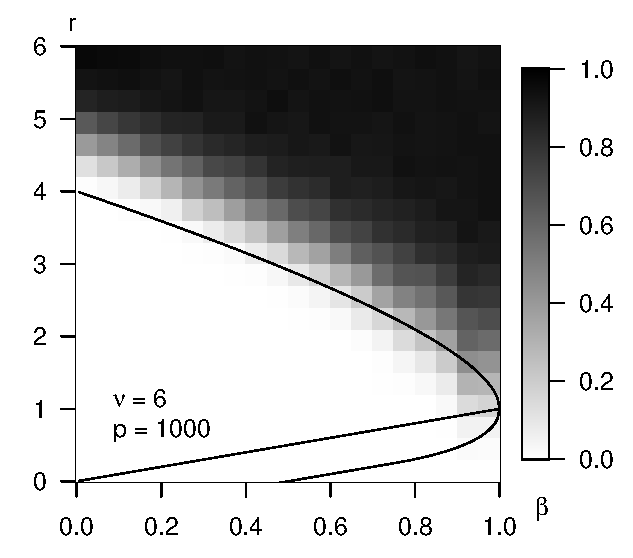
\includegraphics[width=0.32\textwidth]{./sim_strong_boundary/simulated_phase_diagram_chi-squared_nu6_p1000.eps}
      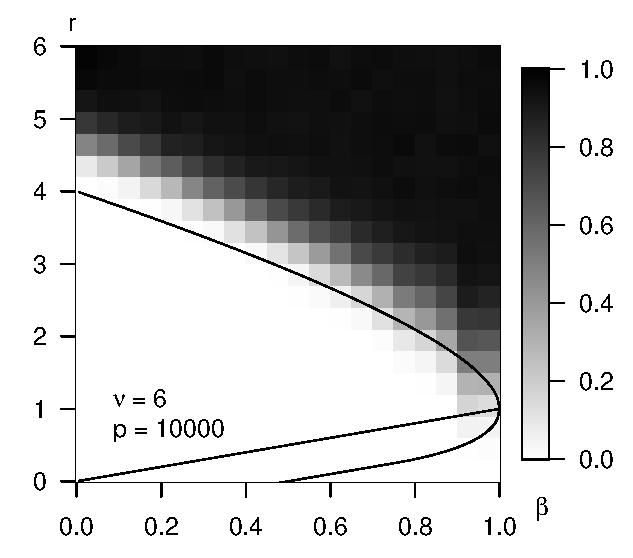
\includegraphics[width=0.32\textwidth]{./sim_strong_boundary/simulated_phase_diagram_chi-squared_nu6_p10000.eps}
      \caption{The empirical probability of exact support recovery using Bonferroni's procedure in the chi-squared model \eqref{eq:model-chisq}. 
      We simulate $\nu=1, 2, 3, 6$ (first to last row), at dimensions $p=100, 1000, 10000$ (left to right column), for a grid of sparsity levels $\beta$ and signal sizes $r$.
      The experiments were repeated 1000 times for each sparsity-signal size combination; darker color indicates higher probability of exact support recovery.  
      Numerical results are generally in agreement with the boundaries described in Theorem \ref{thm:chi-squred-strong-boundary}; for large $\nu$'s and finite dimensions, the phase transitions take place somewhat above the predicted boundaries.
      The weak classification boundary (Theorem \ref{thm:chi-squred-weak-boundary}) and the detection boundary (see \citep{donoho2004higher}) are plotted for comparison.} 
      \label{fig:phase-simulated-chi-squared}
\end{figure}

We conduct further experiments to examine the optimality claims in Theorem \ref{thm:chi-squred-strong-boundary} by applying the oracle procedure with thresholds $t_p=\min_{i\in S}x(i)$.
We also examine the claims Remark \ref{rmk:strong-classification-boundary-1}, and compare the one-sided alternatives in Gaussian additive models with the two-sided alternatives (or equivalently, the chi-square model).
We apply both Bonferroni's procedure and the oracle procedure in both settings.

Experiments were repeated 1000 times for signal sizes ranging from $r=0$ to $6$, and for dimensions 100, 1000, and 10000.
Results of the experiments, shown in Figure \ref{fig:one-vs-two-sided-exact_support_recovery}, suggest vanishing difference between difficulties of two-sided vs one-sided alternatives in the additive error models, as well as vanishing difference between the powers of Bonferroni's procedures and the oracle procedures.

\begin{figure}
      \centering
      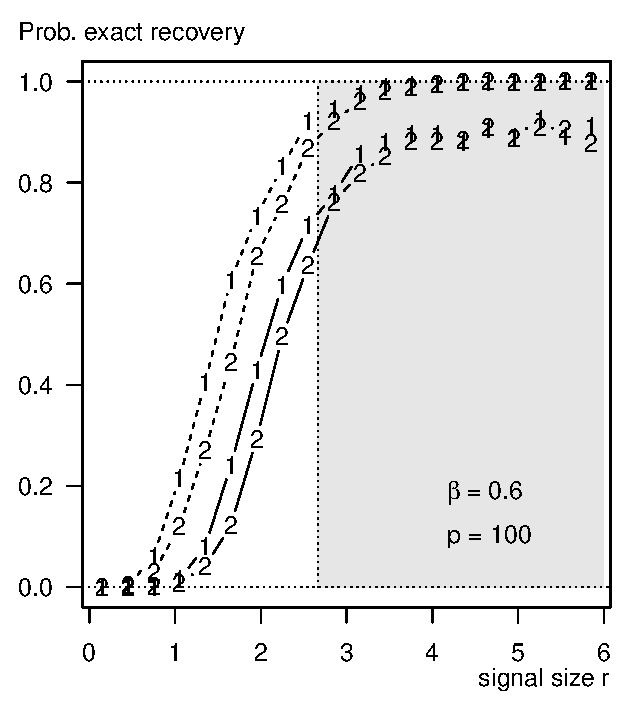
\includegraphics[width=0.32\textwidth]{./sim_one-vs-two-sided/exact_recovery_one-vs-two-sided_beta06_p100.eps}
      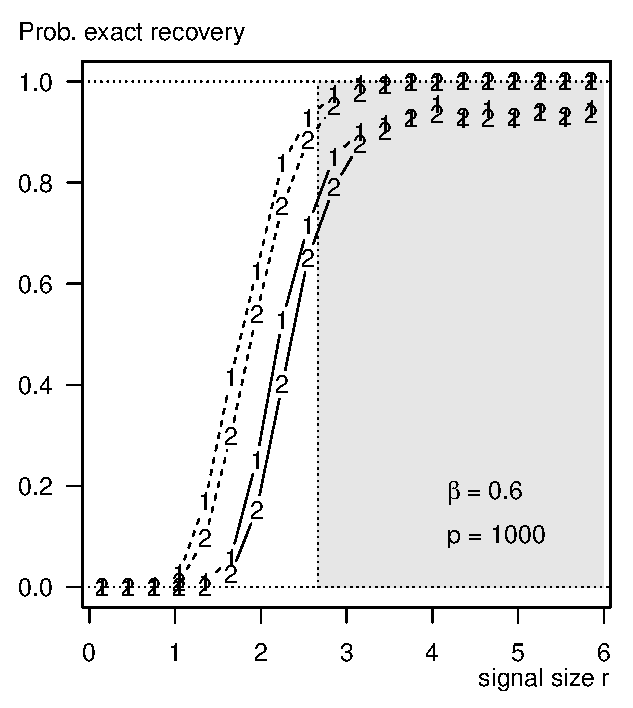
\includegraphics[width=0.32\textwidth]{./sim_one-vs-two-sided/exact_recovery_one-vs-two-sided_beta06_p1000.eps}
      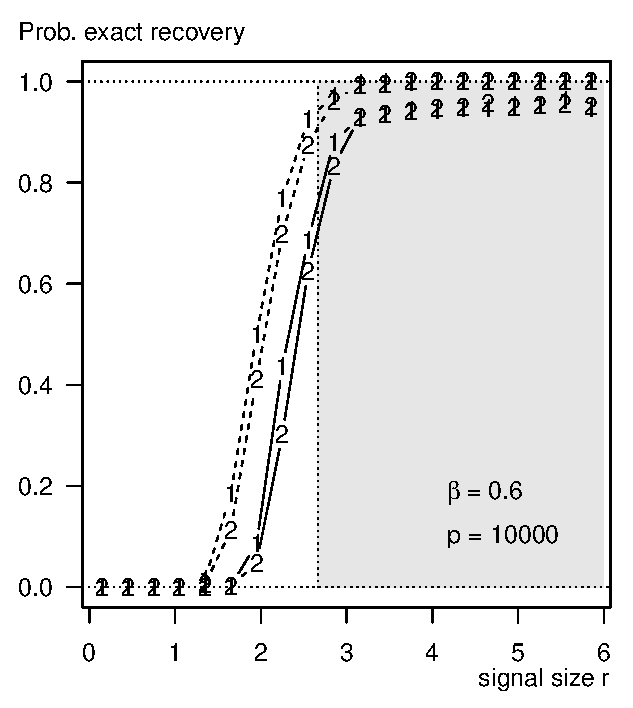
\includegraphics[width=0.32\textwidth]{./sim_one-vs-two-sided/exact_recovery_one-vs-two-sided_beta06_p10000.eps}
      \caption{The empirical probability of exact support recovery using Bonferroni's procedure (solid curves) and the oracle procedure (dashed curves) in the chi-squared model with $\nu=1$ (marked `2') and under one-sided alternatives in the additive Gaussian error model (marked `1'). 
      We simulate at dimensions $p=100, 1000, 10000$ (left to right) for a grid of signal sizes $r$ and sparsity level $\beta=0.6$.
      The experiments were repeated 1000 times for each method-model-signal-size combination. 
      Numerical results show evidence of convergence to the 0-1 law predicted by Theorem \ref{thm:chi-squred-strong-boundary}; regions where exact support recovery is asymptotically achievable are shaded in grey.
      The difference in power between Bonferroni's procedure and the oracle procedure, as well as in the two types of alternatives both decrease as dimensionality increases.} 
      \label{fig:one-vs-two-sided-exact_support_recovery}
\end{figure}

\subsection{The weak classification boundary in finite dimensions}

Similar experiments are conducted to examine the optimality claims in Theorem \ref{thm:chi-squred-weak-boundary}, and in Remark \ref{rmk:weak-classification-boundary}.
The oracle thresholding procedure for approximate support recovery is defined to be the thresholding procedure with threshold
$$
t_p \in \argmin_{t} \frac{|\widehat{S}(t)\setminus S|}{\max\{|\widehat{S}(t)|,1\}} + \frac{|S\setminus \widehat{S}(t)|}{\max\{|{S}|,1\}},
%\mathcal{R^\mathrm{oracle}} \in \argmin_{\widehat{S}(\mathcal{R})\in\mathcal{S}} \mathrm{risk}^{\mathrm{A}}(\mathcal{R}),
$$
where $\widehat{S}(t) = \{i\;|\;x(i)\ge t\}$;
in implementation, we need only scan the observations $t\in\{x(1), \ldots, x(;p)\}$. 
The nominal FDR levels are set at $1/(5{\log{p}})$, in line with the assumptions in Theorem \ref{thm:chi-squred-weak-boundary}; all other parameters are identical to that in the experiments for exact support recovery.
Results of the experiments are shown in Figure \ref{fig:one-vs-two-sided-approx_support_recovery} and Figure \ref{fig:phase-simulated-chi-squared-weak-boundary}.

\begin{figure}
      \centering
      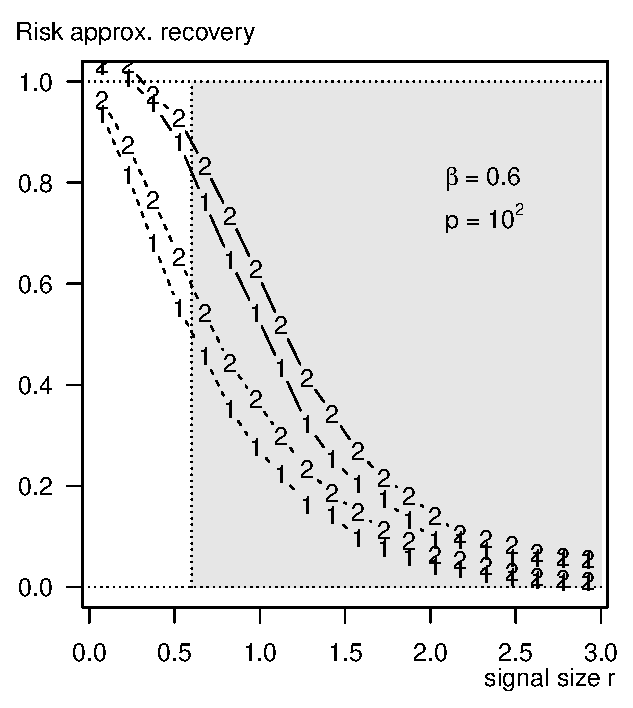
\includegraphics[width=0.32\textwidth]{./sim_one-vs-two-sided/approx_recovery_one-vs-two-sided_beta06_p100.eps}
      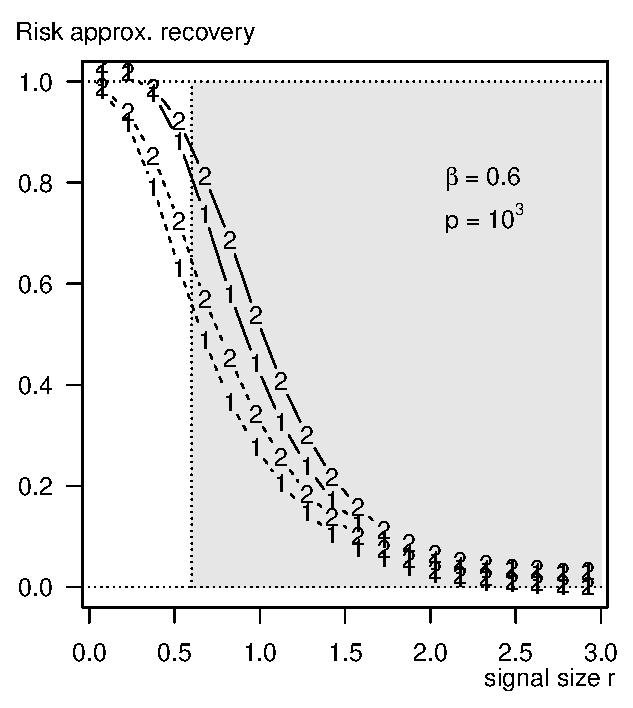
\includegraphics[width=0.32\textwidth]{./sim_one-vs-two-sided/approx_recovery_one-vs-two-sided_beta06_p1000.eps}
      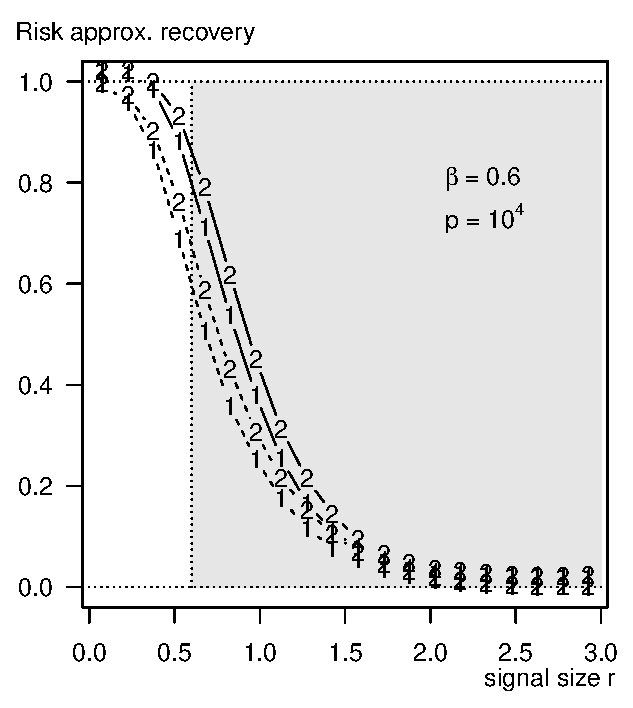
\includegraphics[width=0.32\textwidth]{./sim_one-vs-two-sided/approx_recovery_one-vs-two-sided_beta06_p10000.eps}
      \caption{The empirical risk of approximate support recovery using Benjamini-Hochberg's procedure (solid curves) and the oracle procedure (dashed curves) in the chi-squared model with $\nu=1$ (marked `2') and under one-sided alternatives in the additive Gaussian error model (marked `1'). 
      We simulate at dimensions $p=100, 1000, 10000$ (left to right) for a grid of signal sizes $r$ and sparsity level $\beta=0.6$.
      The experiments were repeated 1000 times for each method-model-signal-size combination. 
      Numerical results show evidence of convergence to the 0-1 law predicted by Theorem \ref{thm:chi-squred-weak-boundary}; regions where approximate support recovery is asymptotically achievable are shaded in grey.
      The difference in power between Benjamini-Hochberg's procedure and the oracle procedure, as well as in the two types of alternatives both decrease as dimensionality increases.} 
      \label{fig:one-vs-two-sided-approx_support_recovery}
\end{figure}


\begin{figure}
      \centering
      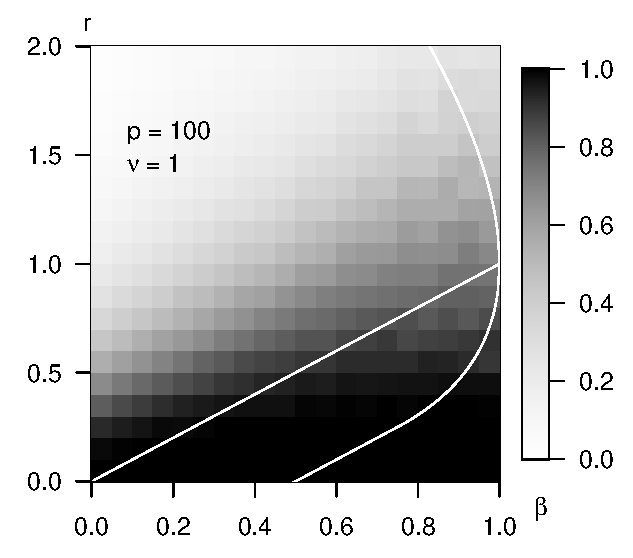
\includegraphics[width=0.32\textwidth]{./sim_weak_boundary/simulated_weak_boundary_chi-squared_nu1_p100.eps}
      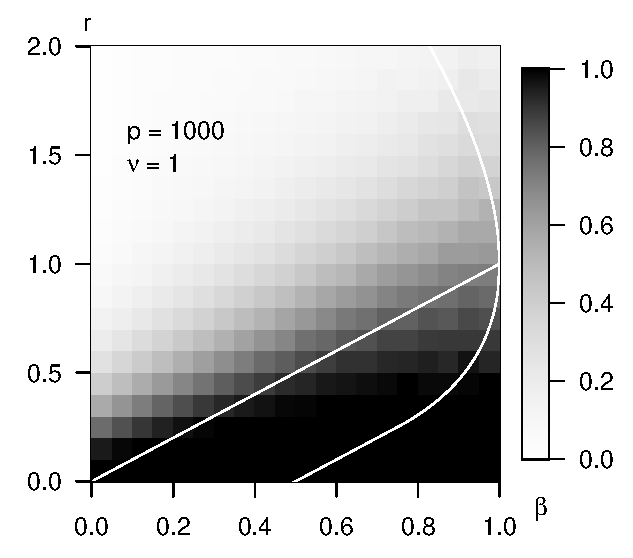
\includegraphics[width=0.32\textwidth]{./sim_weak_boundary/simulated_weak_boundary_chi-squared_nu1_p1000.eps}
      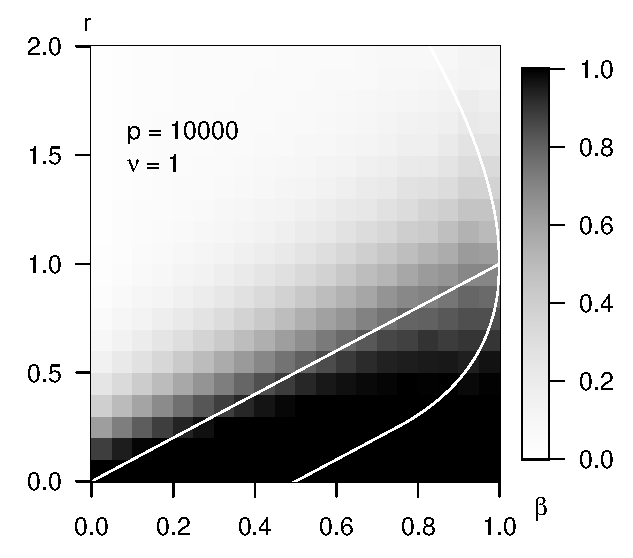
\includegraphics[width=0.32\textwidth]{./sim_weak_boundary/simulated_weak_boundary_chi-squared_nu1_p10000.eps}
      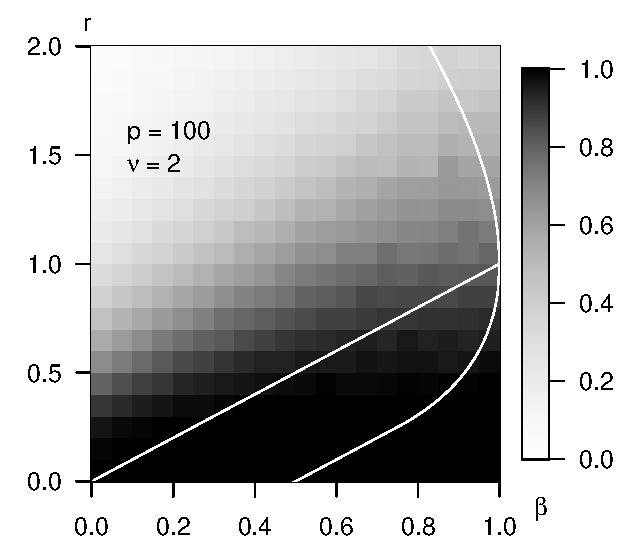
\includegraphics[width=0.32\textwidth]{./sim_weak_boundary/simulated_weak_boundary_chi-squared_nu2_p100.eps}
      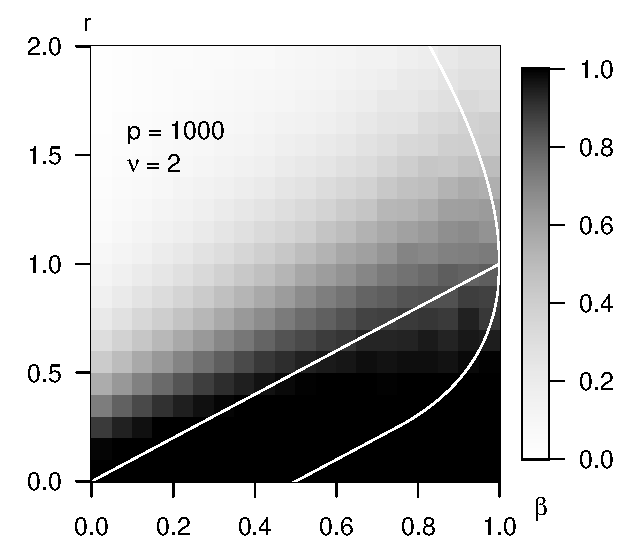
\includegraphics[width=0.32\textwidth]{./sim_weak_boundary/simulated_weak_boundary_chi-squared_nu2_p1000.eps}
      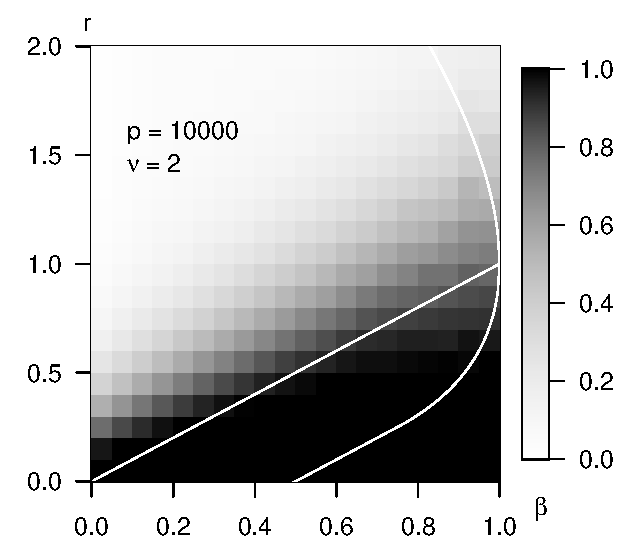
\includegraphics[width=0.32\textwidth]{./sim_weak_boundary/simulated_weak_boundary_chi-squared_nu2_p10000.eps}
      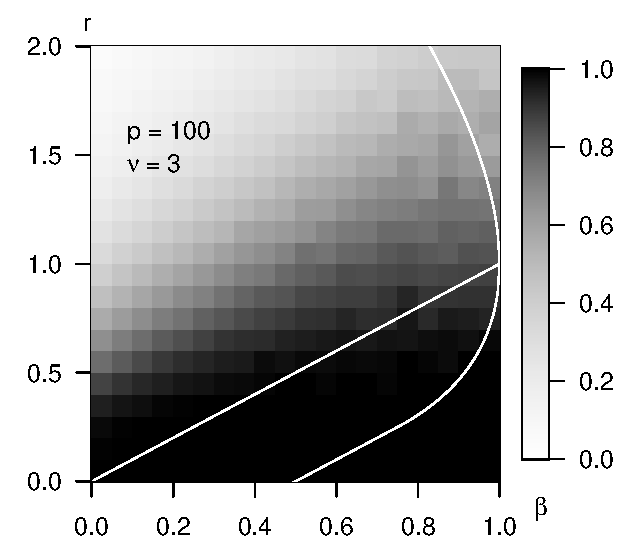
\includegraphics[width=0.32\textwidth]{./sim_weak_boundary/simulated_weak_boundary_chi-squared_nu3_p100.eps}
      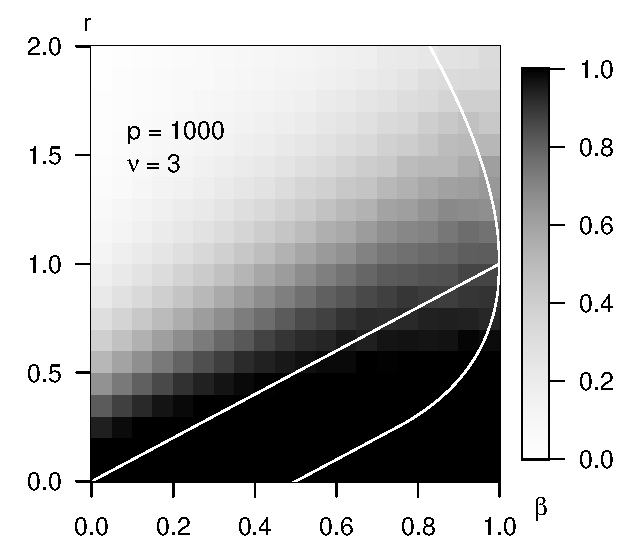
\includegraphics[width=0.32\textwidth]{./sim_weak_boundary/simulated_weak_boundary_chi-squared_nu3_p1000.eps}
      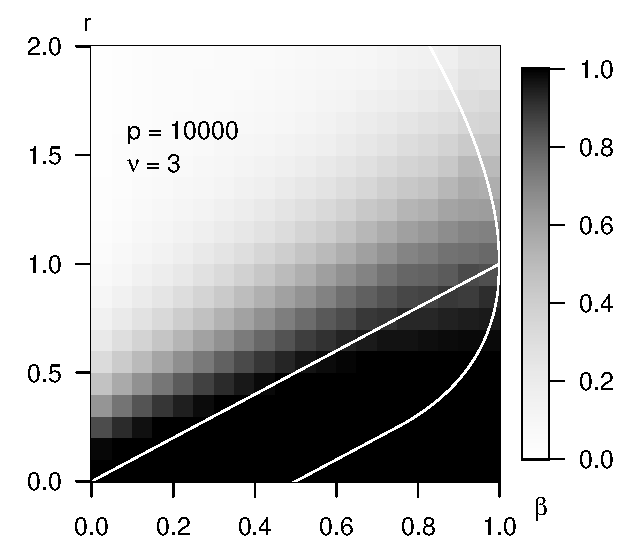
\includegraphics[width=0.32\textwidth]{./sim_weak_boundary/simulated_weak_boundary_chi-squared_nu3_p10000.eps}
      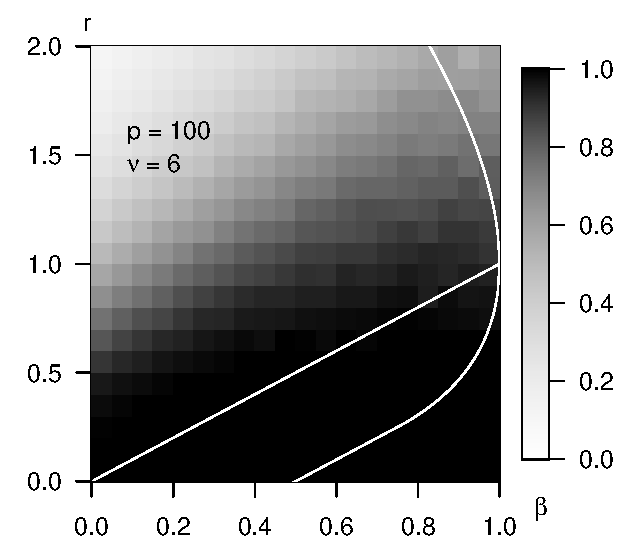
\includegraphics[width=0.32\textwidth]{./sim_weak_boundary/simulated_weak_boundary_chi-squared_nu6_p100.eps}
      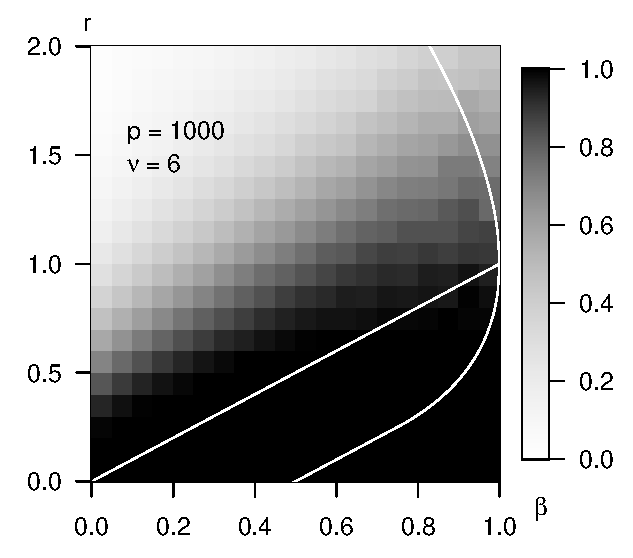
\includegraphics[width=0.32\textwidth]{./sim_weak_boundary/simulated_weak_boundary_chi-squared_nu6_p1000.eps}
      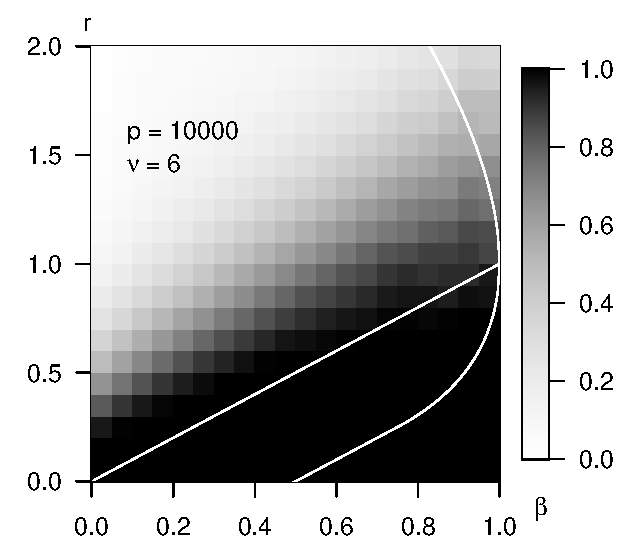
\includegraphics[width=0.32\textwidth]{./sim_weak_boundary/simulated_weak_boundary_chi-squared_nu6_p10000.eps}
      \caption{The estimated risk of approximate support recovery $\mathrm{risk}^{\mathrm{A}}$ (see \eqref{eq:risk-approximate}) of the Benjamini-Hochberg procedure in the chi-squared model \eqref{eq:model-chisq}. 
      We simulate $\nu=1, 2, 3, 6$ (first to last row), at dimensions $p=100, 1000, 10000$ (left to right column), for a grid of sparsity levels $\beta$ and signal sizes $r$.
      The experiments were repeated 1000 times for each sparsity-signal size combination; darker color indicates higher larger $\mathrm{risk}^{\mathrm{A}}$. 
      Numerical results are generally in agreement with the boundaries described in Theorem \ref{thm:chi-squred-weak-boundary}; for large $\nu$'s and finite dimensions, the phase transitions take place somewhat above the predicted boundaries.
      The strong classification boundary (Theorem \ref{thm:chi-squred-strong-boundary}) and the detection boundary (see \citep{donoho2004higher}) are plotted for comparison.} 
      \label{fig:phase-simulated-chi-squared-weak-boundary}
\end{figure}



\subsection{Phase transitions of reported findings from GWAS}